\chapter[Resultados]{Resultados}

	Após a implementação dos \textit{shaders}, foi utilizada a ferramenta \textit{gDEBugger} descrita na Seção \ref{configamb} para fazer medições quanto ao número de quadros por segundo, medida escolhida a fim de avaliar o desempenho para $n$ números de polígonos. Essa medida de desempenho foi adotada para poder avaliar experimentalmente as complexidades algorítmicas dos \textit{shaders} através das curvas plotadas.

	 A   Figura \ref{gdebugger} mostra essa ferramenta sendo utilizada, na qual executa-se o programa e a métrica desejada é mostrada em tempo de execução e também pode ser pode ser exportada no formato CSV.  

	\begin{figure}[h]
	\centering
		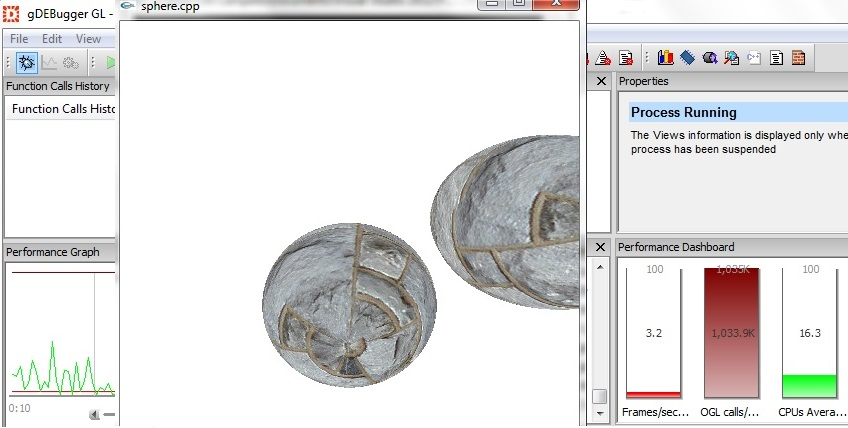
\includegraphics[keepaspectratio=true,scale=0.6]{figuras/gdebugger.jpg}
	\caption{Ferramenta \textit{gDEBugger} sendo utilizada}
	\label{gdebugger}
	\end{figure}

	 Para cada número de subdivisões (no qual foi utilizado o mesmo valor para as subdivisões de latitude e longitude) coletaram-se dez medições, fazendo-se então a média aritmética. O número total de polígonos é dado pela Equação 
(\ref{eqn00}), em que $y$ é o número de polígonos, $s$ é o número de subdivisões e $n$ é a quantidade de esferas. Ao final multiplica-se por dois, pois as subdiviões geram quadriláteros e multiplicando por dois contabilizam-se o número de triângulos (que é o desejado).

	\begin{equation}
	\label{eqn00}
		\mathcal{Y} = s^{2} \cdot n \cdot 2
	\end{equation}

	Assim, as medições foram realizadas, para cada \textit{shader} implementado (\textit{Red, Flatten, Toon, Phong} e  \textit{Texture}). Além disso, variou-se o número de subdivisões das esferas, começando a partir de 50 e incrementando de 25 em 25 até o máximo de subdivisões possíveis, que no caso da esfera utilizada de raio 10, foi de 250. Após este valor, não é possível subdividir mais utilizando as funções da bilblioteca \textit{Glut}. A Tabela \ref{tab01}, Tabela \ref{tab02} e Tabela \ref{tab03} abaixo mostram essas medições, evidenciando a quantidade de quadros pro segundo para determinado número de polígonos.  Estas tabelas foram criadas a fim de poder, posteriormente, plotar os gráficos desejados para a análise de complexidade. 

\begin{table}[h]
	\centering
	\begin{tabular}{cccc}
		\toprule
		\textbf{Nº de subdivisões} & \textbf{Nº de polígonos} 
		& \textbf{\textit{Red Shader}} & \textbf{\textit{Flatten Shader}} \\
		\midrule
		50 & 15000 & 95,2 & 95,4 \\
		75 & 33750 & 49,6  & 47,1\\
		100 & 60000 & 28,6 & 26,3 \\
		125 & 93750 & 18,8  & 18,3 \\
		150 & 135000 & 13,1 & 12,7 \\
		175 & 183750 & 9,6 & 9,4 \\
		200 & 240000 & 7,4 & 7,1 \\
		225 & 303750 & 6,0 & 5,9 \\
		250 & 375000 & 5,2 & 4,9 \\
		\bottomrule
	\end{tabular}
	\caption{Quadros por segundo para o \textit{Red Shader} e o \textit{Flatten Shader}}
	\label{tab01}
\end{table}

\begin{table}[h]
	\centering	
	\begin{tabular}{cccc}
		\toprule
		\textbf{Nº de subdivisões} & \textbf{Nº de polígonos} & 
		\textbf{\textit{Toon Shader}} & \textbf{\textit{Phong Shader}}  \\
		\midrule
		50 & 15000 & 95,2  & 96,6\\
		75 & 33750 & 48,8  & 49,3\\
		100 & 60000 &  28,3 & 28,6\\
		125 & 93750 & 18,1 & 18,4\\
		150 & 135000 &  12,9 & 13,1\\
		175 & 183750 &  9,6 & 9,7\\
		200 & 240000 &  7,5 & 7,4\\
		225 & 303750 &  5,9 & 5,8\\
		250 & 375000 &  5,2 & 5,2\\
		\bottomrule
	\end{tabular}
	\caption{Quadros por segundo para o \textit{Toon Shader} e \textit{Phong Shader}}
	\label{tab02}
\end{table}

\begin{table}[h]
	\centering
	\begin{tabular}{ccc}
		\toprule
		\textbf{Nº de subdivisões} & \textbf{Nº de polígonos} & 
		\textbf{\textit{Texture Shader}}  \\
		\midrule
		50 & 15000 & 76,9  \\
		75 & 33750 & 33,4  \\
		100 & 60000 &  20,3\\
		125 & 93750 & 13,1\\
		150 & 135000 &  9,2\\
		175 & 183750 &  6,8\\
		200 & 240000 &  5,2\\
		225 & 303750 &  4,1\\
		250 & 375000 &  3,4\\
		\bottomrule
	\end{tabular}
	\caption{Quadros por segundo para o \textit{Texture Shader}}
	\label{tab03}
\end{table}

	Com estes dados foi possível traçar as curvas de complexidade algorítmica relativas a cada \textit{texture shader} implementado, tomando como base a quantidade de quadros por segundo. Assim, todas elas foram plotadas em um único gráfico (Figura \ref{complexidade}), que visualmente surege uma curva exponencial decrescente. E com exceção da curva do \textit{texture shader} -- que requer maior poder de processamento -- as curvas dos outros \textit{shaders} ficaram muito próximas, tanto que no gráfico algumas delas tem visualização mais difícil. 

	 \begin{figure}[h]
	\centering
		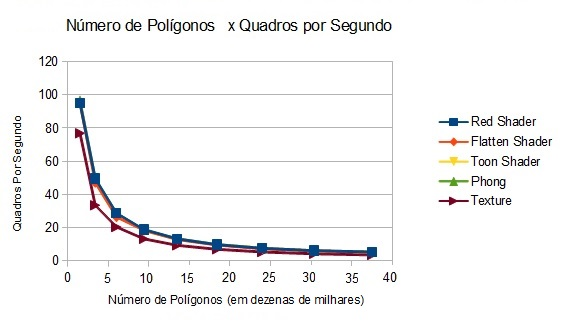
\includegraphics[keepaspectratio=true,scale=0.9]{figuras/complexidade_exp.jpg}
	\caption{Complexidade algoritma: exponencial}
	\label{complexidade}
	\end{figure}

	De acordo com a Seção \ref{metminqua}, foi visto que quando aplica-se a função logarítmica nos dois lados da equação da exponencial, ela se torna uma reta. Assim, para confirmar experimentalmente se a  curva obtida dos gráficos é realmente uma exponencial, traçaram-se os gráficos novamente na Figura \ref{complexidade_reta}, mas dessa vez, na escala logarítmica. 

	\begin{figure}[h]
	\centering
		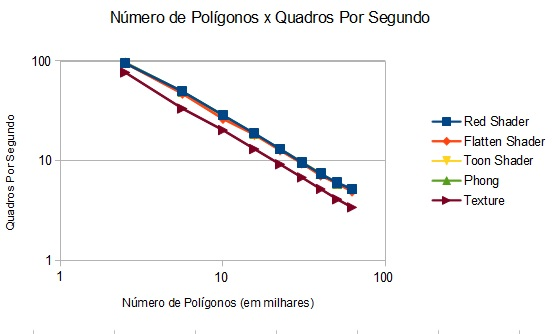
\includegraphics[keepaspectratio=true,scale=0.9]{figuras/complexidade_reta.jpg}
	\caption{\textit{Complexidade Algorítmica: reta}}
	\label{complexidade_reta}
	\end{figure}

	Analisando-se os gráficos, é possível perceber que todos eles se assemelham à uma reta, confirmando as suspeitas levantadas de que a complexidade algorítmica é de ordem exponencial.

\chapter[Conclusão]{Conclusão}
\label{conclusao}

	Através dos experimentos realizados foi possível verificar que é factível desenvolver \textit{shaders} para a plataforma \textit{Android} dentro do prazo estipulado. E por meio da plotagem dos gráficos, a ideia de analisar a complexidade algorítmica experimentalmente mostrou potencial, identificando como ordem de complexidade dos \textit{shaders} uma curva exponencial. Futuramente, mais \textit{shaders} poderão ser analisados e implementados tanto para computador quanto para \textit{Android}, utilizando modelos tridimensionais mais complexos, por meio da leitura do arquivo \textit{obj}. E além disso, com base nas equações extraídas das curvas, o método dos mínimos quadrados -- descrito na Seção \ref{metminqua} -- será utilizado para estimar os parâmetros da curva exponencial específicos de cada \textit{shader}, para cada dispositivo, uma vez que, embora as curvas sejam todas de mesma família, serão justamente estes parâmetros que determinarão as particularidades de cada dispositivo/ambiente. Estas curvas permitirão a estimativa da  quantidade de quadros por segundo dado um número de polígonos. 
	
	Outro ponto importante a que chegou-se foi com relação entre as diferenças da  \textit{OpenGL} e a  \textit{OpenGL ES}, o que ficou evidenciado no momento da conversão de um programa escrito para \textit{mobile} para o computador. O principal aspecto notado foi com relação à remoção das chamadas \texttt{glBegin} e \texttt{glEnd} para desenhar primitivas gráficas e a não utilização do \textit{pipeline} convencional a partir da versão 2.0, em que faz-se obrigatória a utilização de \textit{shaders} pela \textit{OpenGL ES}. Além disso, todo o controle de matrizes de projeção, modelagem (operações de translação, rotação e escalar, por exemplo) e visualização fica a cargo do programador e não mais da \textit{OpenGL ES}. 




